\documentclass[10pt]{article}
\usepackage[T1]{fontenc}
\usepackage[utf8]{inputenc}
\usepackage{lmodern}
\usepackage[margin=0.75in]{geometry}
\usepackage{amsmath,amssymb,booktabs,graphicx,float}
\usepackage{xcolor,listings}
\usepackage[hidelinks]{hyperref}
\graphicspath{{figures/}}
\setlength{\parindent}{0pt}
\setlength{\parskip}{4pt}
\raggedbottom
\setlength{\textfloatsep}{10pt}
\setlength{\intextsep}{10pt}
\setlength{\tabcolsep}{7pt}
\renewcommand{\arraystretch}{1.12}
\renewcommand{\thesection}{Question \arabic{section}}
\newcommand{\prompt}[1]{\begin{quote}\small\itshape #1\end{quote}}
\newcommand{\LN}{\operatorname{LN}}
\newcommand{\RMS}{\operatorname{RMSNorm}}
\newcommand{\GELU}{\operatorname{GELU}}
\newcommand{\SiLU}{\operatorname{SiLU}}
\lstset{basicstyle=\ttfamily\footnotesize,breaklines=true,
  columns=fullflexible,keepspaces=true,showstringspaces=false,
  frame=single,rulecolor=\color{black!20}}
\hypersetup{pdftitle={Mini-LLM Exercise: Five Questions and Experimental Results},
  pdfsubject={Character-level nanoGPT architecture experiments}}
\title{\vspace{-1.6em}Mini-LLM Exercise\\[3pt]
  \large Five Questions and Experimental Results}
\author{}
\date{Experiments conducted on 4 October 2026}

\begin{document}
\maketitle
\vspace{-2em}

\section{Baseline setup}
\prompt{Follow the README's quick-start instructions and train a character-level
language model with the default training configuration
\texttt{config/train\_shakespeare\_char.py}. Plot the training and validation loss.}

The baseline was trained from scratch on the Shakespeare character dataset.
The training split contains 1,003,854 characters, the validation split contains
111,540 characters, and the vocabulary has 65 characters. The default architecture
uses pre-LayerNorm, GELU, learned absolute positional embeddings, and multi-head
attention. It has \textbf{10,745,088 trainable parameters}, counting the tied
token-embedding/output weights once.

The model has 6 layers, 6 attention heads, width 384, and context length 256.
Training uses batch size 64, dropout 0.2, and AdamW with $\beta=(0.9,0.99)$ and
weight decay 0.1. The learning rate follows cosine decay from $10^{-3}$ to
$10^{-4}$ after 100 warmup iterations. Training runs through iteration 5,000
with evaluation every 250 iterations, seed 1337, an RTX 4090, CUDA bfloat16,
PyTorch 2.11.0+cu128, and compilation enabled.

Both plotted losses use evaluation mode, with dropout disabled, averaged over
200 batches per split. Loss is cross-entropy in \textbf{nats per character}; lower
is better. All later experiments use these same training settings and dataset
files, changing one architectural component at a time.

\begin{center}
\small
\begin{tabular}{@{}lrrr@{}}
\toprule
Evaluation & Iteration & Training loss & Validation loss \\
\midrule
Initial & 0 & 4.2874 & 4.2823 \\
Best validation & 1,750 & 1.1045 & 1.4716 \\
Final & 5,000 & 0.6217 & 1.7005 \\
\bottomrule
\end{tabular}
\end{center}

\begin{figure}[H]
\centering
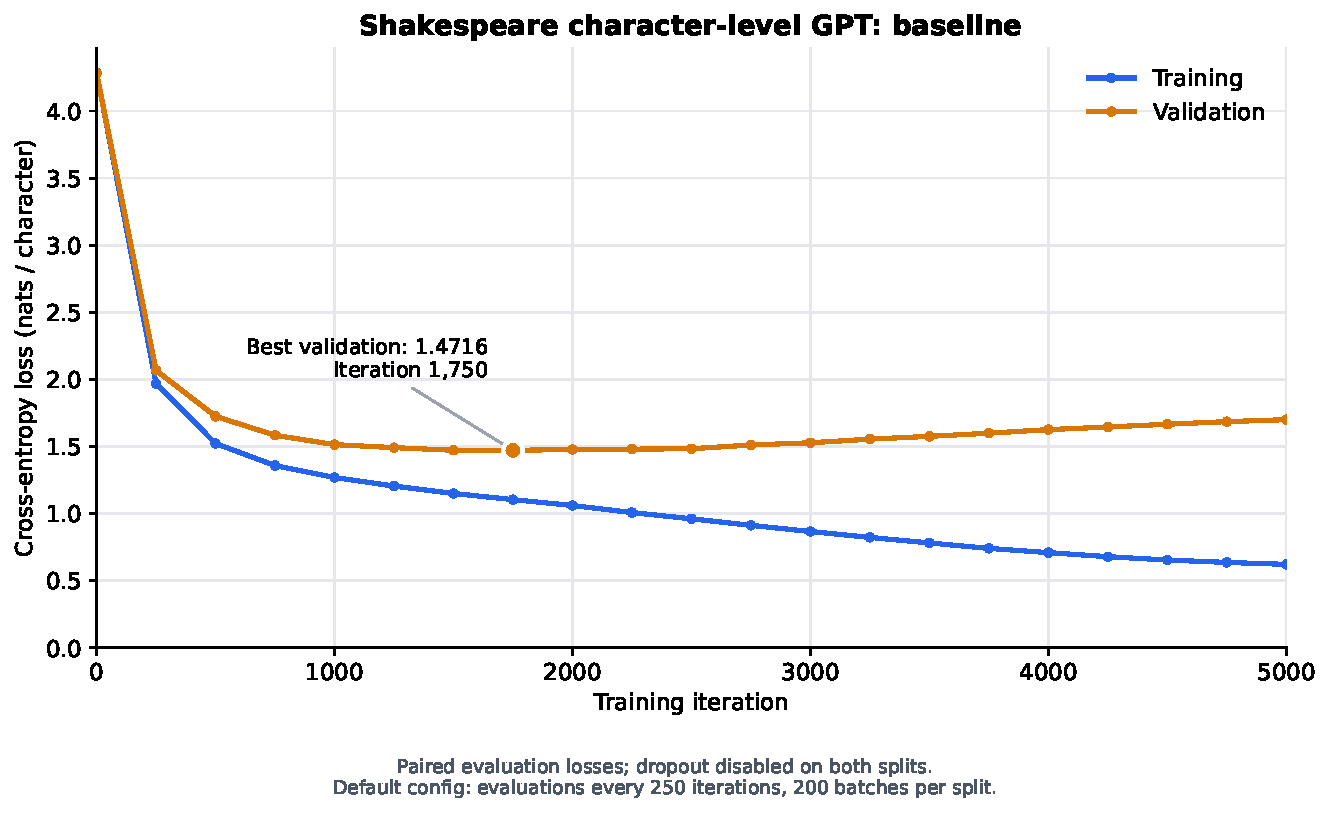
\includegraphics[width=0.62\linewidth]{baseline.pdf}
\caption{Baseline training and validation loss. The best checkpoint is at iteration 1,750.}
\end{figure}

Training loss continues falling after iteration 1,750 while validation loss rises,
indicating overfitting. The saved checkpoint is the one with the lowest validation
loss. The stock training loop includes updates numbered 0 through 5,000; the
evaluation labelled 5,000 occurs before the last update. This convention is the
same in every run.

\clearpage
\section{Effect of LayerNorm}
\prompt{Is the model using pre-LayerNorm or post-LayerNorm? Switch LayerNorm to
RMSNorm, rerun training, and compare the results against the baseline.}

\textbf{The baseline uses pre-LayerNorm.} Each sublayer receives normalized input
before the residual addition:
\begin{align*}
u &= x + \operatorname{Attention}(\LN_1(x)),\\
y &= u + \operatorname{MLP}(\LN_2(u)).
\end{align*}
The final normalization after all Transformer blocks does not change this
pre-norm placement.

All \textbf{13 normalization layers} were replaced by RMSNorm: two per block and
one final normalization. For $x\in\mathbb{R}^{d}$, the implemented normalizations
are
\begin{align*}
\LN(x) &= \gamma\odot\frac{x-\mu}{\sqrt{\frac{1}{d}\sum_{i=1}^{d}(x_i-\mu)^2+\epsilon}},
&\mu&=\frac{1}{d}\sum_{i=1}^{d}x_i,\\
\RMS(x) &= \gamma\odot\frac{x}{\sqrt{\frac{1}{d}\sum_{i=1}^{d}x_i^2+\epsilon}}.
\end{align*}
RMSNorm omits mean subtraction and retains a learned scale~\cite{rmsnorm}.
Both implementations use $\epsilon=10^{-5}$ and no additive bias, consistent with
the baseline's \texttt{bias=False}. Placement and parameter count are unchanged.

\begin{center}
\begin{tabular}{@{}lrr@{}}
\toprule
Metric & LayerNorm baseline & RMSNorm \\
\midrule
Total parameters & 10,745,088 & 10,745,088 \\
Best validation loss & 1.4716 & \textbf{1.4638} \\
Best iteration & 1,750 & 1,750 \\
Final training loss & 0.6217 & 0.6182 \\
Final validation loss & \textbf{1.7005} & 1.7037 \\
\bottomrule
\end{tabular}
\end{center}

\begin{figure}[H]
\centering
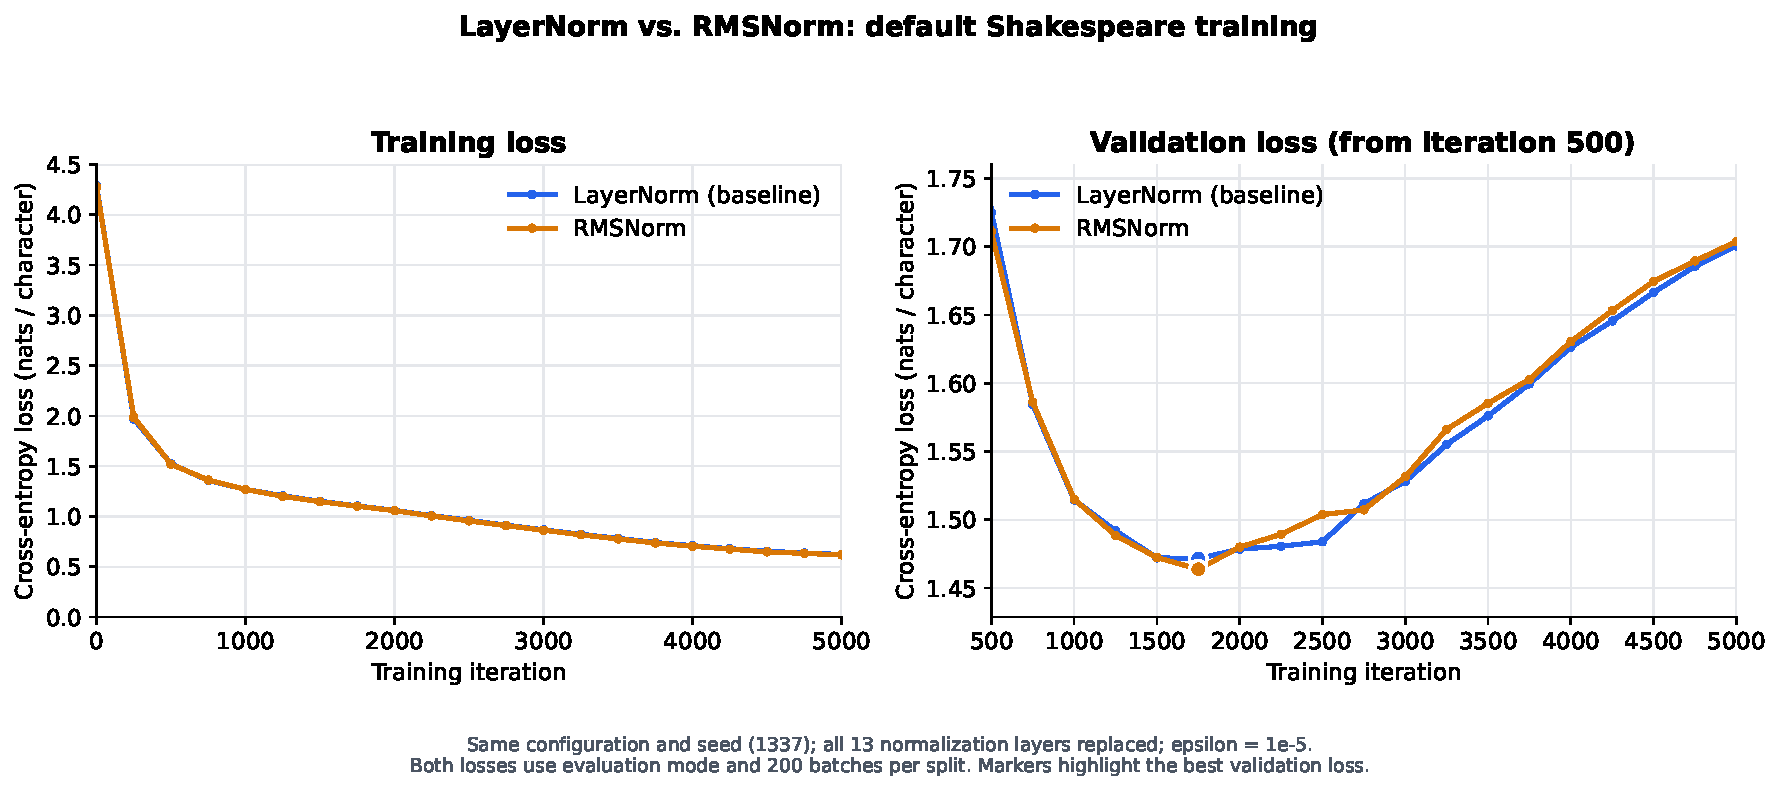
\includegraphics[width=\linewidth]{normalization.pdf}
\caption{LayerNorm versus RMSNorm. The validation panel starts at iteration 500.}
\end{figure}

RMSNorm reduced the best validation loss by $0.0078$ nats/character
(\textbf{0.53\%}) in this run. The training curves are similar, and both runs
overfit after approximately iteration 1,750. RMSNorm's final validation loss is
slightly higher. A single training seed does not establish a consistent advantage.

\clearpage
\section{Effect of the MLP}
\prompt{What activation does the MLP module use? Switch to SwiGLU, keeping roughly
the same parameter count, rerun training, and compare against the baseline.}

\textbf{The baseline MLP uses GELU}, implemented as \texttt{nn.GELU()} with its
default exact formulation. The two linear layers expand width $d=384$ to
$4d=1536$ and project back to $d$.

SwiGLU replaces this computation with a SiLU gate multiplied elementwise by a
second linear projection~\cite{swiglu}:
\begin{align*}
\operatorname{MLP}_{\mathrm{GELU}}(x)
  &= W_{\mathrm{down}}\GELU(W_{\mathrm{up}}x),\\
\operatorname{MLP}_{\mathrm{SwiGLU}}(x)
  &= W_{\mathrm{down}}\bigl[\SiLU(W_{\mathrm{gate}}x)
     \odot(W_{\mathrm{value}}x)\bigr],\\
\SiLU(z)&=z\,\sigma(z).
\end{align*}
The baseline has $2d(4d)=8d^2$ MLP weights. SwiGLU has three matrices and hence
$3dh$ weights. Matching the counts gives
\[
3dh=8d^2\quad\Longrightarrow\quad h=\frac{8d}{3}=\boxed{1024}.
\]
Both MLPs therefore have \textbf{1,179,648 parameters per block}, and both full
models have exactly 10,745,088 parameters. The gate and value projections are
packed into a single linear layer. Pre-LayerNorm, learned positions, attention,
and dropout placement remain as in the baseline.

\begin{center}
\begin{tabular}{@{}lrr@{}}
\toprule
Metric & GELU baseline & SwiGLU \\
\midrule
MLP hidden width & 1,536 & 1,024 \\
Best validation loss & \textbf{1.4716} & 1.4941 \\
Best iteration & 1,750 & 1,500 \\
Final training loss & 0.6217 & 0.5190 \\
Final validation loss & \textbf{1.7005} & 1.8793 \\
\bottomrule
\end{tabular}
\end{center}

\begin{figure}[H]
\centering
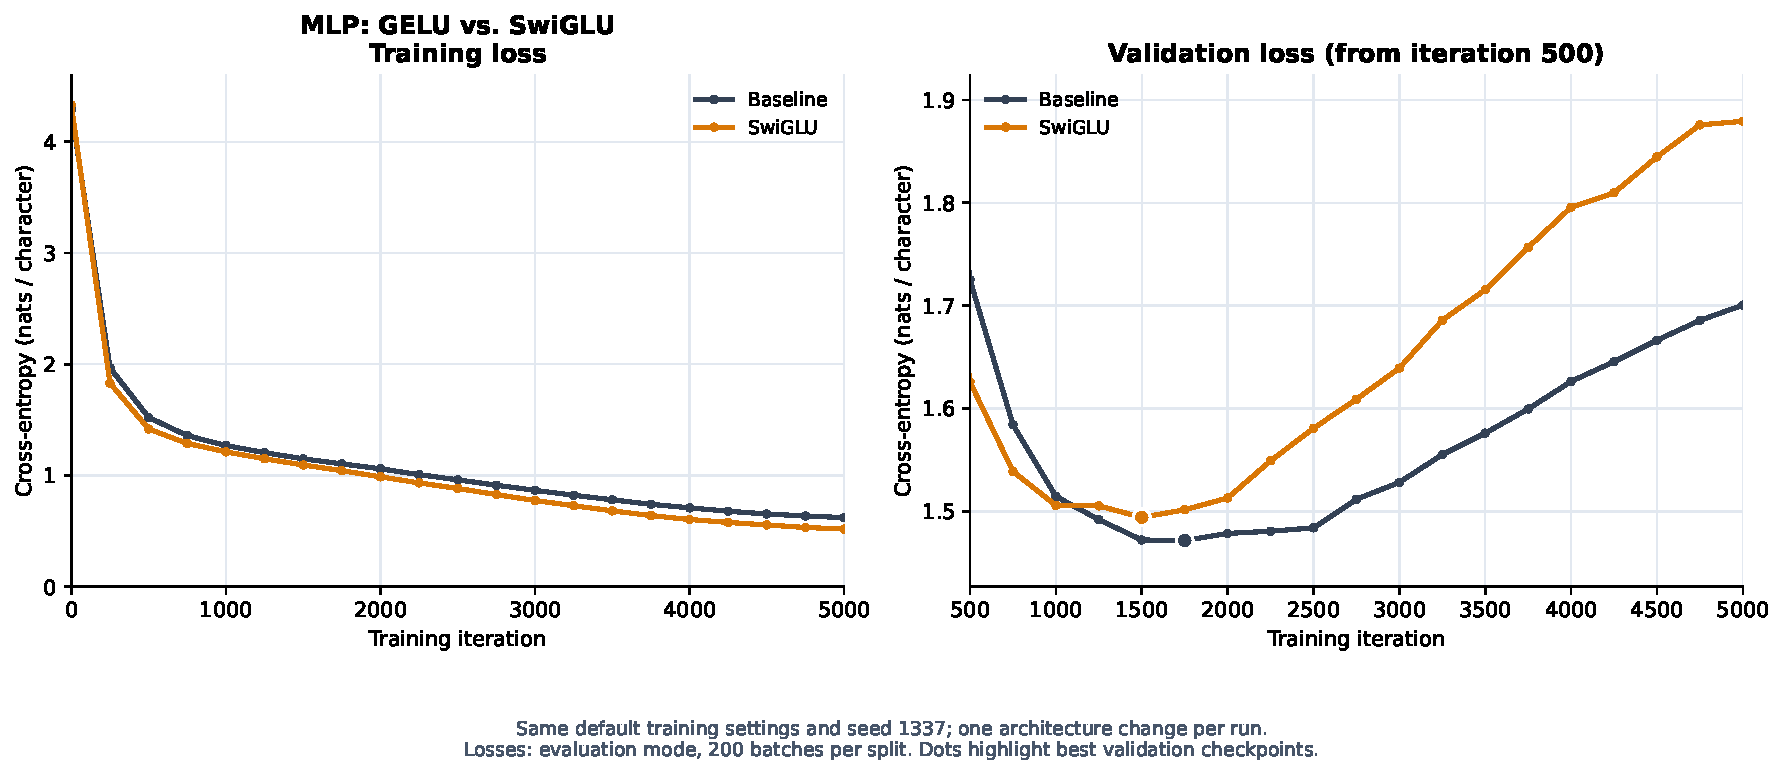
\includegraphics[width=\linewidth]{mlp.pdf}
\caption{GELU versus parameter-matched SwiGLU.}
\end{figure}

SwiGLU fits the training data faster and reaches lower training loss, but its
best validation loss is \textbf{1.53\% higher} than baseline. Its larger final
train/validation gap indicates stronger overfitting under these unchanged
hyperparameters. On identical validation batches, its best checkpoint also
performs worse (1.499301 versus 1.471509; see the shared evaluation below).

\clearpage
\section{Effect of positional encoding}
\prompt{What kind of positional embedding does the model use? Implement
(1) NoPE, removing positional encoding, and (2) RoPE. Rerun training and compare
both variants against the baseline.}

\textbf{The baseline uses learned absolute positional embeddings.} A trainable
table $E_{\mathrm{pos}}\in\mathbb{R}^{256\times384}$ supplies a vector for each
position, added to its token embedding before the first block:
\[
h_t^{(0)}=E_{\mathrm{token}}[s_t]+E_{\mathrm{pos}}[t].
\]
\textbf{NoPE} removes the table and the addition of position vectors. The causal
mask remains, so NoPE removes explicit positional encoding while retaining a
structural source of ordering information.

\textbf{RoPE} also removes the table, but rotates pairs of query and key features
before computing attention scores~\cite{rope}. Values are unchanged. For position
$t$ and feature pair $i$, the head dimension is $d_h=64$ and
\[
\begin{bmatrix}q'_{t,2i}\\q'_{t,2i+1}\end{bmatrix}
=\begin{bmatrix}
\cos(t\omega_i)&-\sin(t\omega_i)\\
\sin(t\omega_i)&\cos(t\omega_i)
\end{bmatrix}
\begin{bmatrix}q_{t,2i}\\q_{t,2i+1}\end{bmatrix},
\qquad \omega_i=10000^{-2i/d_h}.
\]
The same rotation is applied to keys. All 64 head features are rotated; the
trigonometric tables are fixed buffers. Both variants remove $256\times384
=98,304$ learned parameters, leaving \textbf{10,646,784} parameters.

\begin{center}
\small
\begin{tabular}{@{}lrrrr@{}}
\toprule
Positions & Best validation & Best iteration & Final training & Final validation \\
\midrule
Learned baseline & \textbf{1.4716} & 1,750 & 0.6217 & 1.7005 \\
NoPE & 1.5306 & 3,000 & 1.0837 & \textbf{1.5918} \\
RoPE & 1.4731 & 1,750 & 0.5449 & 1.7317 \\
\bottomrule
\end{tabular}
\end{center}

\begin{figure}[H]
\centering
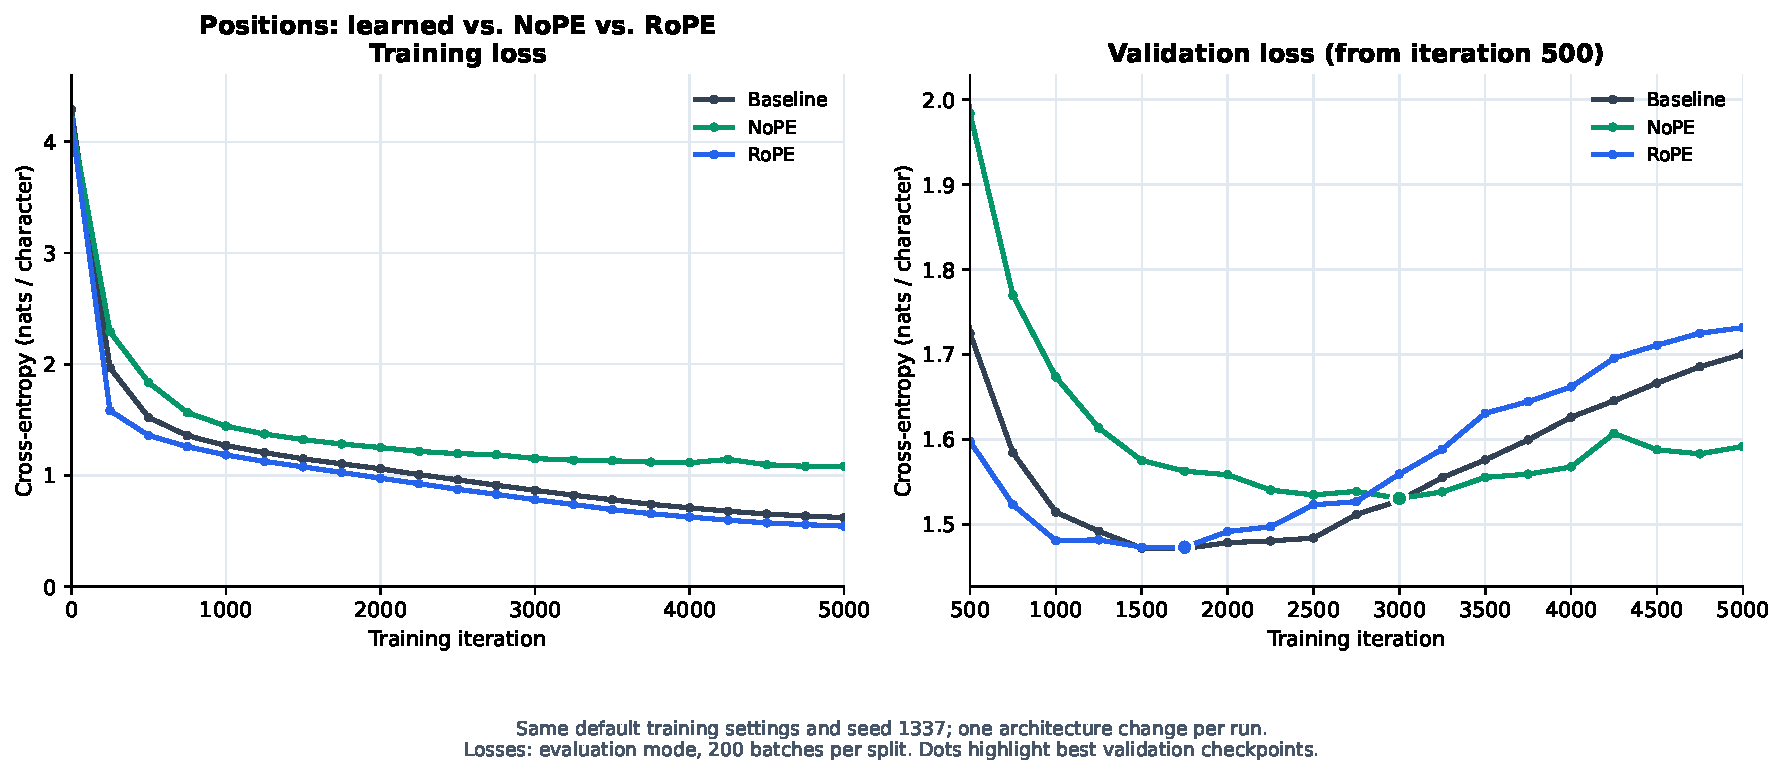
\includegraphics[width=\linewidth]{positions.pdf}
\caption{Learned absolute positions, NoPE, and RoPE.}
\end{figure}

NoPE learns more slowly and its best validation loss is \textbf{4.01\% higher}
than baseline. Its lower final validation loss reflects less overfitting over
this schedule; it does not mean its best checkpoint is better. RoPE learns faster
early on and achieves best validation loss close to baseline ($+0.10\%$).
The shared-batch evaluation slightly favors the baseline. All runs use context
length 256; longer-context generalization was not measured.

\clearpage
\section{Effect of grouped-query attention}
\prompt{The model currently uses multi-head attention. Modify it to use
grouped-query attention with group size 2, so every two query heads share the
same key and value heads. Compare the results against the baseline.}

The baseline uses \textbf{6 query heads, 6 key heads, and 6 value heads}, each of
dimension 64. Grouped-query attention (GQA) keeps all 6 query heads but projects
only \textbf{3 key heads and 3 value heads}~\cite{gqa}. The sharing rule is
\[
\operatorname{KVhead}(j)=\left\lfloor\frac{j}{2}\right\rfloor,
\qquad j\in\{0,1,2,3,4,5\}.
\]
Thus query heads $(0,1)$, $(2,3)$, and $(4,5)$ share their respective K/V heads.
The packed QKV projection changes from $384\rightarrow1152$ to
$384\rightarrow768$. The output projection remains $384\rightarrow384$.
Across six blocks this removes
\[
6\cdot384\cdot(1152-768)=884,736\text{ parameters},
\]
reducing the full model to \textbf{9,860,352 parameters}, or \textbf{8.23\% fewer}.
The implementation uses PyTorch's scaled dot-product attention with
\texttt{enable\_gqa=True}.

\begin{center}
\begin{tabular}{@{}lrr@{}}
\toprule
Metric & MHA baseline & GQA, group size 2 \\
\midrule
Query / key / value heads & 6 / 6 / 6 & 6 / 3 / 3 \\
Total parameters & 10,745,088 & 9,860,352 \\
Best validation loss & 1.4716 & \textbf{1.4692} \\
Best iteration & 1,750 & 2,000 \\
Final training loss & 0.6217 & 0.6307 \\
Final validation loss & 1.7005 & \textbf{1.6863} \\
\bottomrule
\end{tabular}
\end{center}

\begin{figure}[H]
\centering
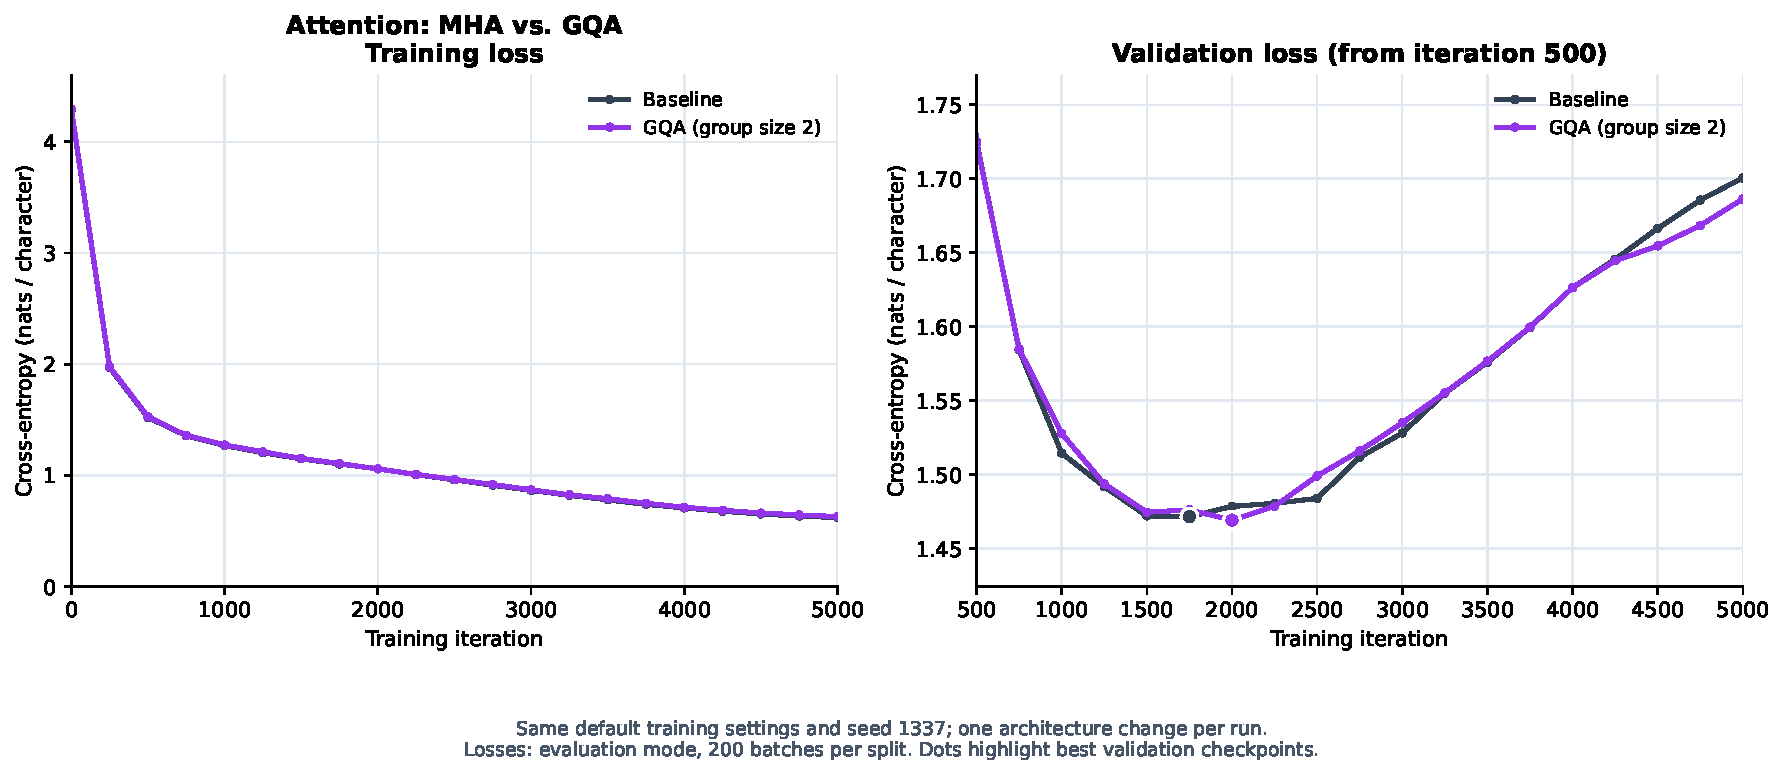
\includegraphics[width=\linewidth]{gqa.pdf}
\caption{Multi-head attention versus GQA with two query heads per K/V head.}
\end{figure}

GQA's best logged validation loss is slightly lower than baseline ($-0.16\%$).
On identical validation windows, this small ranking reverses: GQA scores
1.474026 and baseline scores 1.471509. The supported conclusion is
\textbf{similar validation quality with 8.23\% fewer parameters}. This experiment
does not establish a consistent loss improvement. A decoding KV cache is not
implemented here, so decoding-speed and cache-memory benefits were not measured.

\clearpage
\section*{Shared evaluation and experimental limits}
\addcontentsline{toc}{section}{Shared evaluation and experimental limits}

Every experiment starts from scratch and changes one component of the original
baseline. The SwiGLU, NoPE, RoPE, and GQA variants all retain LayerNorm; they do
not combine the previous RMSNorm change with other modifications.

Architecture changes alter random-number consumption during initialization, so
the same training seed does not guarantee identical weights or minibatch draws.
To improve comparability, the best saved baseline, SwiGLU, NoPE, RoPE, and GQA
checkpoints were also evaluated on \textbf{identical validation windows}: 200
batches of 64 sequences of length 256, with window seed 20261004. This gives
3,276,800 character predictions per checkpoint, using evaluation mode and eager
CUDA bfloat16 execution for all models.

\begin{center}
\begin{tabular}{@{}lrr@{}}
\toprule
Best checkpoint & Shared-window validation loss & Change from baseline \\
\midrule
Baseline & \textbf{1.471509} & --- \\
SwiGLU & 1.499301 & $+1.89\%$ \\
NoPE & 1.535140 & $+4.32\%$ \\
RoPE & 1.477928 & $+0.44\%$ \\
GQA, group size 2 & 1.474026 & $+0.17\%$ \\
\bottomrule
\end{tabular}
\end{center}

RMSNorm was not included in this additional shared-window evaluation; its
comparison in Question 2 uses the original training-log evaluations. The shared
windows may overlap and come from the existing validation split, so they do not
constitute an independent test dataset.

All experiments use one training seed. The results support conclusions about
these runs, without establishing statistical significance across seeds. In
particular, the small differences for RMSNorm, RoPE, and GQA need additional
training seeds to establish reliable gains. The reported losses are rounded to
four decimals in the training logs and six decimals in the additional evaluation.

\textbf{Verification.} All runs completed successfully. Fifteen automated checks
passed, covering baseline compatibility, normalization, SwiGLU parameter counts,
RoPE identities and a separate attention reference, GQA outputs and gradients
against tied-head MHA, causality, checkpoint restoration, cropping, and generation.
Actual saved checkpoints were loaded and verified, and the shared evaluation
completed for all five checkpoints listed above.

\begin{thebibliography}{9}
\raggedright
\bibitem{rmsnorm}
\emph{Root Mean Square Layer Normalization}. arXiv:1910.07467.
\url{https://arxiv.org/abs/1910.07467}.
\bibitem{swiglu}
\emph{GLU Variants Improve Transformer}. arXiv:2002.05202.
\url{https://arxiv.org/abs/2002.05202}.
\bibitem{rope}
\emph{RoFormer: Enhanced Transformer with Rotary Position Embedding}.
arXiv:2104.09864. \url{https://arxiv.org/abs/2104.09864}.
\bibitem{gqa}
\emph{GQA: Training Generalized Multi-Query Transformer Models from Multi-Head
Checkpoints}. arXiv:2305.13245. \url{https://arxiv.org/abs/2305.13245}.
\end{thebibliography}

\clearpage
\section*{Reproduction and included files}

The source code and full experiment artifacts are in the nanoGPT project.
All newly created scripts, reports, logs, checkpoints, and figures are under
\texttt{nanoGPT-master/Mini-LLM Exercise}. Each run includes its configuration,
source snapshot, dataset hashes, training log, and best checkpoint.

The independent architecture options, applied to
\texttt{config/train\_shakespeare\_char.py}, are:
\begin{center}
\small
\begin{tabular}{@{}ll@{}}
\toprule
Experiment & Training option \\
\midrule
Baseline & Defaults \\
RMSNorm & \texttt{--norm\_type=rmsnorm} \\
SwiGLU & \texttt{--mlp\_type=swiglu} \\
NoPE & \texttt{--pos\_encoding=nope} \\
RoPE & \texttt{--pos\_encoding=rope} \\
GQA & \texttt{--kv\_group\_size=2} \\
\bottomrule
\end{tabular}
\end{center}

Use a separate output directory for each training run. For the four architecture
variants, the runner handles these paths automatically. From \texttt{nanoGPT-master}:
\begin{lstlisting}
python3 -u -B 'Mini-LLM Exercise/run_architecture_experiments.py'
python3 -B 'Mini-LLM Exercise/evaluate_architecture_checkpoints.py'
python3 -B 'Mini-LLM Exercise/compare_architectures.py'
\end{lstlisting}
Completed runs are skipped by the runner. Pass \texttt{--run-tag repeat1} to
create fresh architecture runs, and use the same tag for their evaluation and
comparison scripts.

Regenerate the baseline and normalization plots, or run the checks:
\begin{lstlisting}
python3 -B 'Mini-LLM Exercise/plot_training_loss.py'
python3 -B 'Mini-LLM Exercise/compare_normalization.py'
python3 -B -m unittest discover -s 'Mini-LLM Exercise' -p 'test_*.py' -v
\end{lstlisting}

This portable report package contains the \LaTeX{} source, compiled PDF, five
vector PDF figures, and the numerical summaries and CSV data used in the report.
From the extracted report folder, compile with:
\begin{lstlisting}
latexmk -pdf -interaction=nonstopmode -halt-on-error \
  -outdir=build mini_llm_exercise.tex
\end{lstlisting}
The generated PDF will be \texttt{build/mini\_llm\_exercise.pdf}. On Overleaf,
upload the ZIP package and select \texttt{mini\_llm\_exercise.tex} as the main
document, with pdfLaTeX as the compiler.

\end{document}
